\documentclass{article}

\usepackage[utf8]{inputenc}
\usepackage[brazil]{babel}

\title{Estudo Dirigido: Perceptron Simples}
\author{Rúbia Reis Guerra \\ 2013031143}

\usepackage{Sweave}
\begin{document}
\Sconcordance{concordance:perceptron.tex:perceptron.rnw:%
1 8 1 1 0 11 1 1 2 1 0 1 1 1 4 2 0 2 1 1 4 2 0 1 3 1 0 1 1 1 5 3 0 1 1 %
1 2 5 0 1 2 1 1 1 3 2 0 1 1 1 2 1 0 2 1 4 0 1 2 3 1 1 4 3 0 2 1 1 3 1 0 %
1 11 10 0 1 4 2 0 1 1 1 2 1 0 2 1 4 0 1 2 3 1 1 5 4 0 1 3 1 0 1 1 4 0 1 %
2 2 1}

\maketitle

\section{Perceptron Simples}
No contexto de redes neurais, um perceptron é um neurônio artificial que utiliza a função degrau de Heaviside como função de ativição. A atividade proposta teve como objetivo o estudo e a implementação de um perceptron de camada única, que corresponde à rede neural \textit{feedforward} mais simples existente.

\section{Implementação}

\subsection{Funções \textit{yperceptron} e \textit{trainperceptron}}
Para esta atividade, foi proposta a implementação das funções \textit{yperceptron}, correspondente à função de ativação degrau do Percepetron, e \textit{trainperceptron}, que calcula e ajusta o vetor de pesos por correção de erros, descritas nas notas de aula disponibilizadas.
\begin{Schunk}
\begin{Sinput}
> rm(list=ls())
> library('plot3D')
> ##############################################
> # Cálculo da resposta do neurônio #
> # (função degrau) #
> yperceptron <- function(xvec, w, par)
+ {
+   if(par == 1)
+     xvec <- cbind(-1, xvec)
+   u <- xvec %*% w
+   y <- 1*(u >= 0)
+   return(as.matrix(y))
+ }
> ##############################################
> # Treinamento de um Perceptron simples #
> # (ajuste do vetor de pesos) #
> trainperceptron <- function(xin, yd, eta, tol, maxepocas, par)
+ {
+   dimxin <- dim(xin)
+   N <- dimxin[1]
+   n <- dimxin[2]
+   if(par == 1)
+   {
+     wt <- as.matrix(runif(n+1) - 0.5)
+     xin <- cbind(-1, xin)
+   }
+   else 
+   {
+     wt <- as.matrix(runif(n) - 0.5)
+   }
+   
+   nepocas <- 0
+   eepoca <- tol+1
+   evec <- matrix(nrow=1, ncol=maxepocas)
+   
+   while ((nepocas < maxepocas) && (eepoca > tol))
+   {
+     ei2 <- 0
+     xseq <- sample(N)
+     for(i in 1:N)
+     {
+       irand <- xseq[i]
+       yhati <- as.double((xin[irand,] %*% wt) >= 0)
+       ei <- yd[irand]- yhati
+       dw <- eta*ei*xin[irand,]
+       wt <- wt+dw
+       ei2 <- ei2+ei*ei
+     }
+     nepocas <- nepocas+1
+     evec[nepocas] <- ei2/N
+     eepoca <- evec[nepocas]
+   }
+   retlist <- list(wt=wt, evec=evec[1:nepocas])
+   return(retlist)
+ }
\end{Sinput}
\end{Schunk}

\subsection{Parâmetros e amostragem de dados}
Os dados foram amostrados de duas distribuições de bivariadas ($x_{1}$,$x_{2}$), caracterizadas por $\mathcal{N}(2,2,\sigma^2)$ e $\mathcal{N}(4,4,\sigma^2)$. Os parâmetros foram definidos em:
\begin{itemize}
\item Tamanho da população (N): 100
\item Passo de atualização de $w$ (eta): 0.1
\item Tolerância (tol): 0.01
\item Número máximo de épocas (maxepocas): 10000
\item Adição de bias a x (par): TRUE
\item Limites do grid (minseq, maxseq): (0,6)
\end{itemize}
\begin{Schunk}
\begin{Sinput}
> ##############################################
> # Parâmetros #
> N <- 200
> minseq <- 0
> maxseq <- 6
> eta <- 0.1
> tol <- 0.01
> maxepocas <- 10000
> par <- 1
> s1 <- 0.4
> s2 <- 0.4
> ##############################################
> # Gerando dados amostrados das distribuições #
> # m1=(2,2)', m2=(4,4)' #
> xc1 <- matrix(rnorm(N*2),ncol=2)*s1+t(matrix((c(2,2)),ncol=N,nrow=2))
> xc2 <- matrix(rnorm(N*2),ncol=2)*s2+t(matrix((c(4,4)),ncol=N,nrow=2))
> xin <- rbind(xc1,xc2)
> ##############################################
> # Rótulos das entradas #
> yd <- rbind(matrix(0, nrow=N, ncol=1), matrix(1, nrow=N, ncol=1))
> ##############################################
> # Plot dos dados #
> plot(xc1[,1], xc1[,2], col='red', type='p', xlim=c(minseq,maxseq), 
+      ylim=c(minseq,maxseq), xlab='x_1', ylab='x_2',
+      sub = 'Dados amostrados')
> par(new=T)
> plot(xc2[,1], xc2[,2], col='blue', type='p', xlim=c(minseq,maxseq), 
+      ylim=c(minseq,maxseq), xlab='', ylab='')
\end{Sinput}
\end{Schunk}
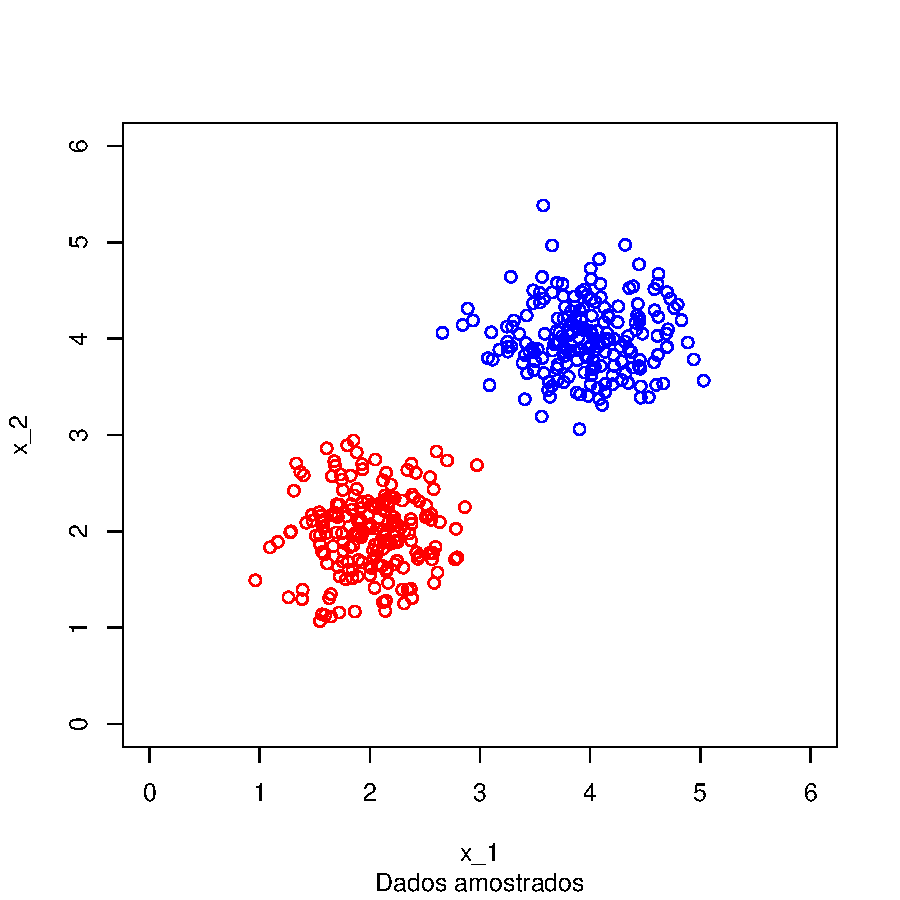
\includegraphics{perceptron-002}

\subsection{Treinamento}
Para encontrar o vetor de pesos $w$, realiza-se o treinamento do Perceptron simples utilizando os parâmetros definidos previamente.
\begin{Schunk}
\begin{Sinput}
> ##############################################
> # Treinamento #
> train <- list()
> train <- trainperceptron(xin,yd,eta,tol,maxepocas,par)
> # Vetor de pesos #
> w <- train$wt
> paste(w)
\end{Sinput}
\begin{Soutput}
[1] "1.91799562298693"  "0.355739361358345" "0.286721633603696"
\end{Soutput}
\end{Schunk}

\subsection{Superfície de Separação}
Encontrado o vetor de pesos $w$, implmenta-se a função \textit{yperceptron} percorrendo o espaço $R^2$.
\begin{Schunk}
\begin{Sinput}
> ##############################################
> # Mapeamento do grid  #
> seqi <- seq(minseq,maxseq,0.1)
> seqj <- seq(minseq,maxseq,0.1)
> M <- matrix(1,nrow =length(seqi),ncol=length(seqj))
> # Percorrer o espaço e gerar a saída #
> ci <- 0
> for (i in seqi)
+ {
+   ci <- ci+1
+   cj <- 0
+   for (j in seqj)
+   {
+     cj <- cj + 1
+     xt <- c(i,j)
+     M[ci,cj] <- yperceptron(t(xt),w,1)
+   }
+ }
\end{Sinput}
\end{Schunk}

\subsection{Resposta do Perceptron Simples}
\begin{Schunk}
\begin{Sinput}
> ##############################################
> # Resposta em R2 #
> plot(xc1[,1], xc1[,2], col='red', type='p', xlim=c(minseq,maxseq), 
+      ylim=c(minseq,maxseq),xlab='x_1',ylab='x_2',
+      sub = 'Resposta do Perceptron Simples')
> par(new=T)
> plot(xc2[,1], xc2[,2], col='blue', type='p', xlim=c(minseq,maxseq), 
+      ylim=c(minseq,maxseq),xlab='',ylab='')
> par(new=T)
> contour(seqi,seqj,M,xlim=c(minseq,maxseq), 
+      ylim=c(minseq,maxseq),xlab='',ylab='')
\end{Sinput}
\end{Schunk}
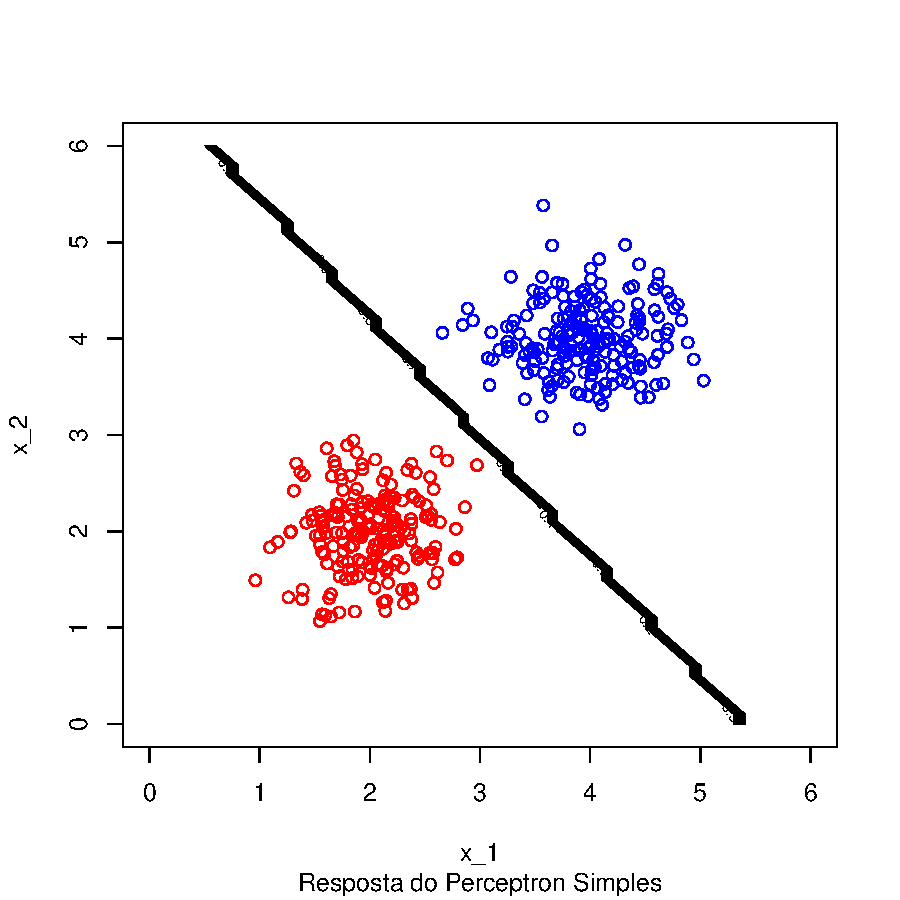
\includegraphics{perceptron-005}

Plot da superfície de separação gerada pela função perceptron:
\begin{Schunk}
\begin{Sinput}
> ##############################################
> #Superfície de separação #
> persp(seqi,seqj,xlim=c(0,6),ylim=c(0,6),M,theta=-20,phi=80,
+       sub='Superfície de separação')
\end{Sinput}
\end{Schunk}
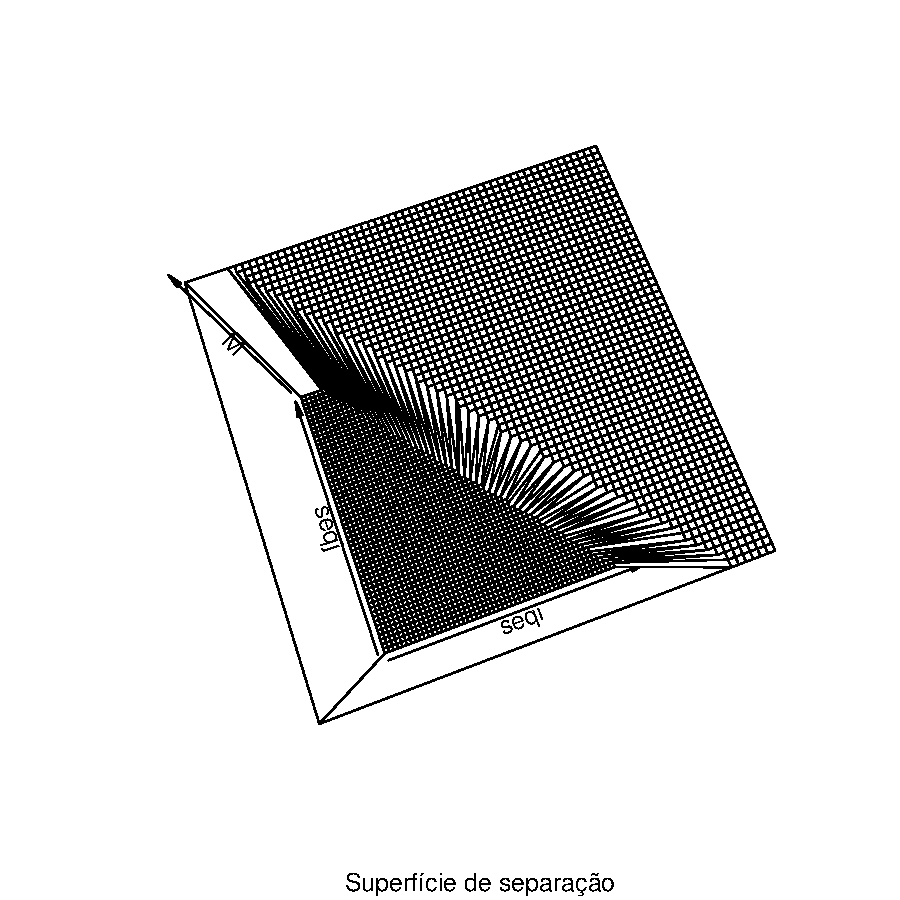
\includegraphics{perceptron-006}

\begin{Schunk}
\begin{Sinput}
> ##############################################
> # Superfície de separação + dados amostrados #
> ribbon3D(seqi,seqj,M, xlim=c(minseq,maxseq), ylim=c(minseq,maxseq), 
+          zlim=c(0,1), contour=T, add=F, axes=T, ticktype="detailed",
+          sub='Superfície de separação')
> # Dados #
> scatter3D(xc1[,1],xc1[,2], matrix(0,nrow=dim(xc1)[1]),add=T,col='red')
> scatter3D(xc2[,1],xc2[,2], matrix(0,nrow=dim(xc2)[1]),add=T,col='blue')
\end{Sinput}
\end{Schunk}
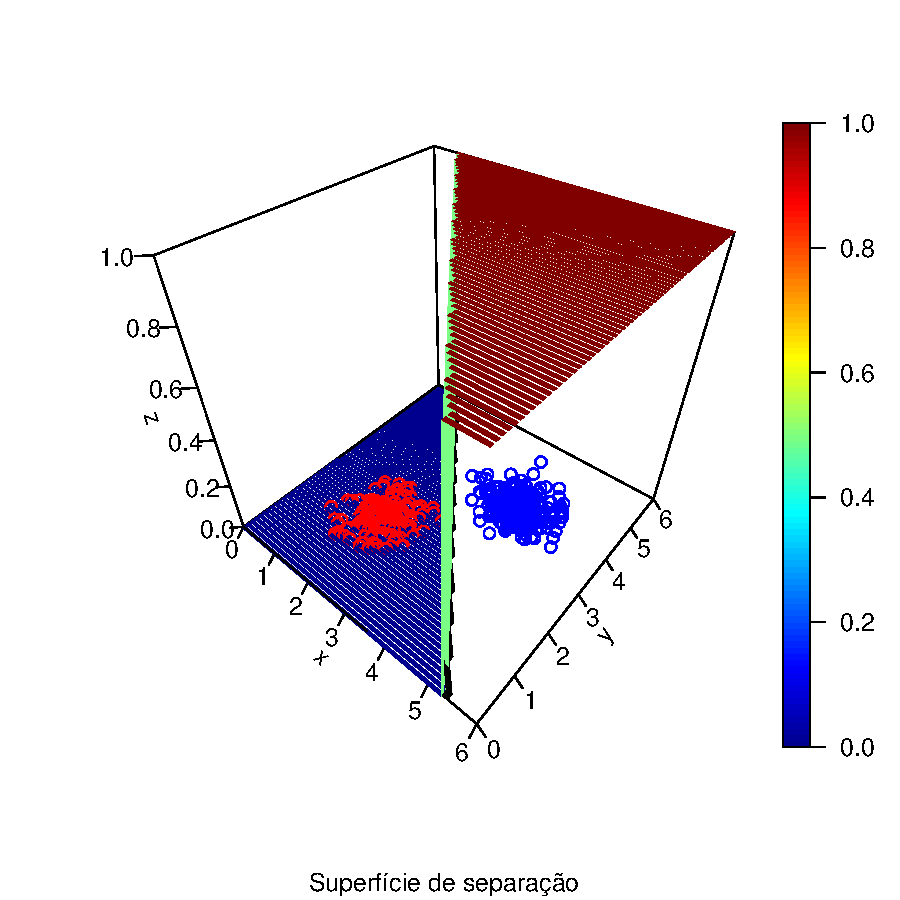
\includegraphics{perceptron-007}


\end{document}
